\subsection{\texorpdfstring{空间 \(\mathcal{L}_{\mathrm{F}}^{\infty}\)}{空间 L sub F to infinity}}

定义 2. --- 对 X 到一个 Banach 空间 F 中的每个映射 f，令 \(\mathrm{N}_{\infty}(\mathbf{f}) = \mathrm{M}_{\infty}(|\mathbf{f}|)\)；称 f（对测度 \(\mu\) ）是依测度有界的，如果 \(\mathrm{N}_{\infty}(\mathbf{f})\) 有限。X 到 F 中的可测且依测度有界的映射所成之集记作 \(\mathcal{L}_{\mathrm{F}}^{\infty}(\mathrm{X}, \mu)\)（或 \(\mathcal{L}_{\mathrm{F}}^{\infty}(\mu)\)，或简记为 \(\mathcal{L}_{F}^{\infty}\)）。

于是函数 \(\mathbf{f}\)（\(\mathcal{L}_{\mathrm{F}}^{\infty}\) 中的）可如此刻画：存在一个局部几乎处处等于 \(\mathbf{f}\) 的有界可测函数。

由 (1) 立即得出

\[
\mathrm{N} _ {\infty} (\mathbf {f} + \mathbf {g}) \leqslant \mathrm{N} _ {\infty} (\mathbf {f}) + \mathrm{N} _ {\infty} (\mathbf {g});
\]

另一方面，\(\mathrm{N}_{\infty}(\alpha\mathbf{f}) = |\alpha| \mathrm{N}_{\infty}(\mathbf{f})\) 对每个标量 \(\alpha\) 成立。因此集合 \(\mathcal{L}_{F}^{\infty}\) 是 X 到 F 中的全体映射所成空间的一个线性子空间，且 \(\mathrm{N}_{\infty}(\mathbf{f})\) 是这个向量空间上的一个半范数。设 \((\mathbf{f}_{n})\) 是 \(\mathcal{L}_{F}^{\infty}\) 中函数的一个序列，它收敛于 \(f \in \mathcal{L}_{F}^{\infty}\)（对由半范数 \(\mathrm{N}_{\infty}(\mathbf{f})\) 定义的拓扑）；对每个整数 m，存在一个局部可忽略集 \(H_{m}\) 与一个整数 \(n_{0}\)，使 \(|\mathbf{f}(x) - \mathbf{f}_{n}(x)| \leqslant 1/m\) 对每个整数 \(n \geqslant n_{0}\) 与每个 \(x \notin H_{m}\) 成立（可数个局部可忽略集的并是局部可忽略的）；诸 \(H_{m}\) 之并 H 是局部可忽略的，而且可以看出，在局部可忽略集 H 的补集上，\(\mathbf{f}_{n}(x)\) 一致收敛于 \(\mathbf{f}(x)\)；反之亦然。

显然，每个与 \(\mathcal{L}_{F}^{\infty}\) 中的函数局部几乎处处相等的函数都属于 \(\mathcal{L}_{F}^{\infty}\) 。特别地，X 上以 F 为值的局部可忽略函数构成一个线性子空间 \(\mathcal{N}_{F}^{\infty}\)（\(\mathcal{L}_{F}^{\infty}\) 中的），由关系式 \(\mathrm{N}_{\infty}(\mathbf{f}) = 0\) 刻画（即 0 在由 \(\mathrm{N}_{\infty}(\mathbf{f})\) 定义的拓扑中的闭包）。与 \(\mathcal{L}_{F}^{\infty}\) 相伴的 Hausdorff 空间，即商空间 \(\mathcal{L}_{\mathrm{F}}^{\infty}/\mathcal{N}_{\mathrm{F}}^{\infty}\)，记作 \(\mathrm{L}_{\mathrm{F}}^{\infty}(\mathrm{X}, \mu)\)（或 \(\mathrm{L}_{\mathrm{F}}^{\infty}(\mu)\) 或 \(\mathrm{L}_{\mathrm{F}}^{\infty}\)）；其拓扑由从 \(N_{\infty}\) 过渡到商所得到的范数定义；类 \(\dot{f} \in L_{F}^{\infty}\) 的范数记作 \(\mathrm{N}_{\infty}(\dot{f})\)，也记作 \(\|f\|_{\infty}\) 。当 F = R（相应地，C）时，若不致引起混淆，我们写 \(\mathcal{L}^{\infty}\) 与 \(L^{\infty}\) 以代替 \(\mathcal{L}_{R}^{\infty}\) 与 \(L_{R}^{\infty}\)（相应地，\(\mathcal{L}_{C}^{\infty}\) 与 \(L_{C}^{\infty}\)）。

命题 2. --- 空间 \(\mathcal{L}_{\mathrm{F}}^{\infty}\) 是完备的；空间 \(\mathrm{L}_{\mathrm{F}}^{\infty}\) 是一个 Banach 空间。

因为，设 \((\mathbf{f}_{n})\) 是 \(\mathcal{L}_{F}^{\infty}\) 中的一个 Cauchy 序列；对每个整数 n，存在整数 \(k_{n}\)，使 \(\mathrm{N}_{\infty}(\mathbf{f}_{r}-\mathbf{f}_{s})\leqslant1/n\) 对 \(r\geqslant k_{n}\) 与 \(s\geqslant k_{n}\) 成立；于是存在一个局部可忽略集 \(A_{rs}\)，使 \(|\mathbf{f}_{r}(x)-\mathbf{f}_{s}(x)|\leqslant1/n\) 对所有 \(x\notin A_{rs}\) 成立 。若 \(A_{n}\) 是诸集 \(A_{rs}\)（对 \(r\geqslant k_{n}\) 与 \(s\geqslant k_{n}\)）之并，则 \(A_{n}\) 局部可忽略，且对每个 \(x\notin A_{n}\)，\(|\mathbf{f}_{r}(x)-\mathbf{f}_{s}(x)|\leqslant1/n\) 对所有指标 \(r\geqslant k_{n}\)、\(s\geqslant k_{n}\) 成立 。设 A 是诸 \(A_{n}\) 之并所成的局部可忽略集，并令 \(\mathbf{g}_{n}(x)=\mathbf{f}_{n}(x)\)（对 \(x\notin A\)），\(\mathbf{g}_{n}(x)=0\)（对 \(x\in A\)）；则 \(g_{n}\) 属于 \(\mathcal{L}_{F}^{\infty}\)，且由 A 的定义，序列 \((\mathbf{g}_{n})\) 在 X 上一致收敛于一个函数 g。由此推出函数 g 可测（§5, No.~4, 定理 2）；此外，g 在由 \(x\in X\)（在那里 \(|\mathbf{g}_{k_{1}}(x)|\leqslant\mathrm{N}_{\infty}(\mathbf{g}_{k_{1}})\)）所成之集上有界，且由于该集的补集局部可忽略，故 g 属于 \(\mathcal{L}_{F}^{\infty}\) 。显然，在 \(\mathcal{L}_{F}^{\infty}\) 中，序列 \((\mathbf{g}_{n})\) 以 g 为极限，因而序列 \((\mathbf{f}_{n})\) 亦然，因为对所有 n 有 \(\mathrm{N}_{\infty}(\mathbf{f}_{n}-\mathbf{g}_{n})=0\) 。~命题的第二部分可由此立即推出。

注. --- 1) 每个有界连续函数 \(\mathbf{f}\)（\(X\) 上以 \(F\) 为值的）属于 \(\mathcal{L}_{\mathrm{F}}^{\infty}\)，且

\[
\mathrm{N} _ {\infty} (\mathbf {f}) \leqslant \| \mathbf {f} \| = \sup _ {x \in \mathrm{X}} | \mathbf {f} (x) |.
\]

为使对每个有界连续函数 f 有 \(\mathrm{N}_{\infty}(\mathbf{f})=\|\mathbf{f}\|\)，其充要条件是测度 \(\mu\) 的支集等于 X。因为，若存在一个具有可忽略紧支集且不恒为零的连续函数 f，则 \(\mathrm{N}_{\infty}(\mathbf{f})=0\) 而 \(\|f\|>0\) 。反之，若 \(\mu\) 的支集等于 X，则对每个有界连续函数 f 与每个数 \(\alpha<\|f\|\)，由 \(x\in X\)（满足 \(|\mathbf{f}(x)|>\alpha\) 者）所成之集是开且非空的，故其外测度 \textgreater0，这就表明 \(\mathrm{N}_{\infty}(\mathbf{f})=\|\mathbf{f}\|\) 。

于是，当 \(\mu\) 的支集等于 \(X\) 时，我们可以把赋范空间 \(\mathcal{C}^b (X;F)\)——即 \(X\) 上以 \(F\) 为值的有界连续函数所成的——与空间 \(\mathcal{L}_{F}^{\infty}\) 的一个子空间等同起来。由于 \(\mathcal{L}_F^\infty\) 一般不是 Hausdorff 的，子空间 \(\mathcal{C}^b (X;F)\) 在 \(\mathcal{L}_F^\infty\) 中一般不是闭的，但它在 \(L_F^\infty\) 中的规范像是 \(L_F^\infty\) 的一个闭子空间（在所考虑的情形下它还可以与 \(\mathcal{C}^b (X;F)\) 等同）。一般说来，\(\mathcal{C}^b (X;F)\) 与 \(L_F^\infty\) 不同，也就是说，对任意的有界可测函数 \(\mathbf{f}\)，一般不存在连续函数 \(\mathbf{g}\)（局部几乎处处等于 \(\mathbf{f}\) 者）（ \(\S 5\) , 习题 12）。这蕴涵：空间 \(\mathcal{K}(X;F)\)（由 \(X\) 到 \(F\) 中的具有紧支集的连续映射组成）在 \(L_F^\infty\) 中一般不稠密，而它在每个空间 \(L sub F to the p\)（ \(1\leqslant p < +\infty\)）中都稠密（ \(\S 3\) , No.~4. 定义 2）。

\pandocbounded{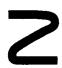
\includegraphics[keepaspectratio]{images/part002_fffac8d3.jpg}}

\begin{enumerate}
\def\labelenumi{\arabic{enumi})}
\setcounter{enumi}{1}
\tightlist
\item
  显然，由半范数 \(N_{\infty}\) 定义的拓扑细于依测度收敛的拓扑在 \(L_{F}^{\infty}\) 上诱导的拓扑（§5, No.~11）。
\end{enumerate}

